\documentclass[tikz, border=1mm]{standalone}

\usetikzlibrary{positioning}

\begin{document}
	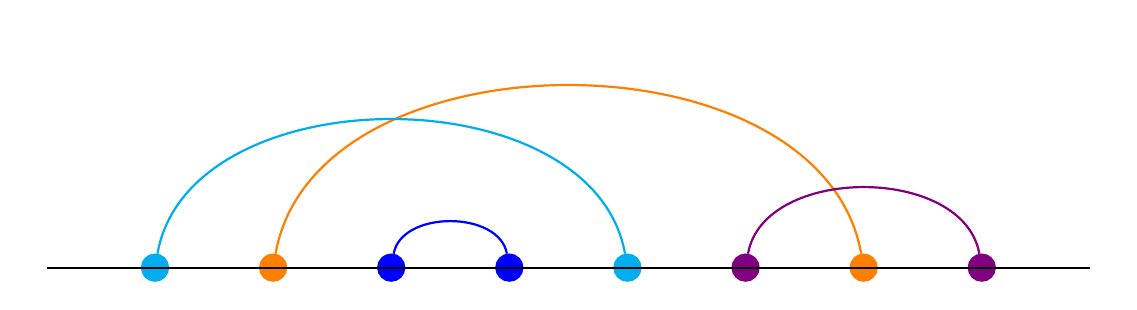
\begin{tikzpicture}[node distance={15mm}, thick, main/.style = {draw, circle, fill}]
		\node (L) {};
		\node[main, color=cyan] (1) [right of=L] {};
		\node[main, color=orange] (2) [right of=1] {};
		\node[main, color=blue] (3) [right of=2] {};
		\node[main, color=blue] (4) [right of=3] {};
		\node[main, color=cyan] (5) [right of=4] {};
		\node[main, color=violet] (6) [right of=5] {};
		\node[main, color=orange] (7) [right of=6] {};
		\node[main, color=violet] (8) [right of=7] {};
		\node (R) [right of=8] {};
		\draw[main] (L) edge (R);
		\draw[bend left=80, color=orange] (2) edge (7);
		\draw[bend left=80, color=violet] (6) edge (8);
		\draw[bend left=80, color=blue] (3) edge (4);
		\draw[bend left=80, color=cyan] (1) edge (5);
	\end{tikzpicture}
\end{document}